%%%%%%%%%%%%%%%%%%%%%%%%%%%%%%%%%%%%%%%%%%%%%%%%%%%%%%%%%%%%%%%%%
%%% %
%%% % weiiszablon.tex
%%% % The Faculty of Electrical and Computer Engineering
%%% % Rzeszow University Of Technology diploma thesis Template
%%% % Szablon pracy dyplomowej Wydziału Elektrotechniki 
%%% % i Informatyki PRz
%%% % June, 2015
%%%%%%%%%%%%%%%%%%%%%%%%%%%%%%%%%%%%%%%%%%%%%%%%%%%%%%%%%%%%%%%%%

\documentclass[12pt,twoside]{article}

\usepackage{weiiszablon}

\author{Rafał Stępień}

\studentID{EF-169625}

\title{Książkowy dziennik w chmurze}
\titleEN{Cloud-based book journal}

\newcommand{\rodzajPracyNo}{1}


\supervisor{dr inż. Mariusz Mączka}

\supervisorEN{Dr. Eng. Mariusz Mączka}

\abstract{Treść streszczenia po polsku}
\abstractEN{Treść streszczenia po angielsku}

\begin{document}

\maketitle

\blankpage

\tableofcontents

\clearpage
\blankpage

\section{Wstęp}
W dobie rosnącej cyfryzacji i dynamicznego rozwoju technologii mobilnych, coraz więcej osób poszukuje
nowoczesnych narzędzi wspierających codzienne czynności, w tym także zarządzanie swoimi pasjami i 
zainteresowaniami. Jedną z takich pasji, cieszącą się niezmienną popularnością, jest czytanie książek.
Wraz z rosnącą liczbą dostępnych tytułów zarządzanie osobistą biblioteką może stać się problematyczne.

Niniejsza praca dotyczy zaprojektowania i implementacji aplikacji mobilnej o nazwie 
„BookTracker”, stworzonej z wykorzystaniem technologii Jetpack Compose 
oraz zintegrowanej z internetową bazą danych Supabase. Aplikacja oferuje użytkownikom możliwość 
oznaczania książek jako posiadanych lub przeczytanych, śledzenia nadchodzących premier 
literackich oraz zarządzania osobistą biblioteką w sposób przejrzysty i dostępny z każdego 
miejsca, dzięki wykorzystaniu technologii chmurowych. Tematyka ta została wybrana ze względu 
na rosnącą popularność aplikacji wspierających organizację życia codziennego oraz potrzebę 
zapewnienia użytkownikom narzędzi umożliwiających wygodne i efektywne zarządzanie ich kolekcjami 
literackimi.

Zakres pracy obejmuje zaprojektowanie kluczowych funkcji aplikacji, implementację interfejsu 
użytkownika oraz integrację z bazą danych w chmurze. Głównym celem pracy jest stworzenie aplikacji mobilnej, 
która w przejrzysty sposób umożliwi użytkownikom zarządzanie osobistą biblioteką książek z 
wykorzystaniem technologii chmurowych.

\clearpage

\section{Podobne aplikacje}

W dzisiejszych czasach niemal każda aplikacja ma już swoje odpowiedniki na rynku. Podczas 
tworzenia aplikacji postawiono więc na skupienie się na grupie docelowej użytkowników, którzy
oczekują konkretnych rozwiązań.

\subsection{Bookmory}

Bookmory to przykład wielu istniejących aplikacji dzięki którym można zarządzać swoją biblioteką, do jej
odpowiedników można zaliczyć jeszcze kilka aplikacji takich jak: StoryGraph, Bookshelf, czy Bookly.
Każda z wymienionych aplikacji spełnia podobne zadania, a dla większości użytkowników wybór pomiędzy nimi
nie ma większego znaczenia, ponieważ różnice między nimi są minimalne.

Istnienie tych aplikacji zainspirowało stworzenie alternatywy, która będzie różniła się od swoich
poprzedników unikalną funkcjonalnością i skupieniem się na konkretnej grupie odbiorców.

\subsection{TV Time}

TV Time to popularna aplikacja służąca do śledzenia postępu oglądania seriali i filmów. 
Pomimo tego, że aplikacja ta nie ma możliwości zarządzania książkami i skupia się wyłącznie na 
produkcjach filmowych, to funkcjonalność śledzenia seriali stała się inspiracją do stworzenia
alternatywnej aplikacji do śledzenia postępu czytania książek. Główną różnicą do 
istniejących już rozwiązań jest skupienie się na seriach książek wydawanych w tomach i ułatwieniu
użytkownikom obserwowania i zarządzania książkami, które są ze sobą powiązane.

\clearpage

\section{Środowiska i technologie}

Wybór odpowiednich środowisk i technologii jest kluczowym elementem każdego projektu informatycznego, 
ponieważ wpływa zarówno na efektywność pracy, jak i na jakość końcowego rozwiązania. Ważnym jest 
przedstawienie wybranych rozwiązań i uzasadnienie dlaczego były one wybrane zamiast alternatywnych
opcji.

\subsection{Android Studio}

Android Studio to oficjalne zintegrowane środowisko programistyczne (IDE) do tworzenia aplikacji na system
Android bazujące na IntelliJ IDEA firmy JetBrains, stworzone i rozwijane przez firmę Google. Jest to 
kompleksowe narzędzie, które oferuje zestaw funkcji, mających na celu ułatwienie tworzenia, debugowania i
publikowania aplikacji.

Środowisko to jest nieustannie aktualizowane przez Google, aby wspierać najnowsze wersje systemu Android
oraz dodawać nowe funkcje. Android Studio obsługuje programowanie w językach takich jak Java, Kotlin 
(rekomendowany przez Google), a także w mniejszym stopniu w C++.

Kluczowym elementem jest edytor kodu, który obsługuje autouzupełnianie, refaktoryzację oraz podpowiedzi 
kontekstowe, co znacząco ułatwia pisanie czystego i efektywnego kodu.

Android Studio zostało wybrane ze względu na to, że jest najpełniejszym narzędziem do tworzenia aplikacji
na system android i w przeciwieństwie do np. Visual Studio Code, można praktycznie od razu rozpocząć
pracę zamiast zajmowania się instalowaniem rozszerzeń i potrzebnych komponentów. Android Studio oferuje 
wszystkie niezbędne funkcje w jednym pakiecie.

\subsection{Kotlin}

Kotlin to nowoczesny, statycznie typowany język programowania, który został stworzony przez firmę 
JetBrains i jest oficjalnie wspierany przez Google do tworzenia natywnych aplikacji na system Android. 
Kotlin jest zaprojektowany z myślą o prostocie, bezpieczeństwie i interoperacyjności z Javą - język ten 
jest w pełni kompatybilny z istniejącym ekosystemem Javy, co umożliwia łatwą integrację z istniejącym kodem i 
bibliotekami.

Kotlin oferuje wiele nowoczesnych funkcji, które czynią go atrakcyjnym wyborem. Jego kluczowe 
cechy to m.in. zwięzła składnia, która pozwala na pisanie czytelnego i mniej podatnego na błędy kodu, oraz 
zaawansowane mechanizmy, takie jak obsługa funkcji wyższych rzędów, rozszerzenia klas czy programowanie funkcyjne. 
Wbudowane mechanizmy bezpieczeństwa, takie jak system typów zapobiegający błędom typu null pointer exception 
(tzw. "null safety"), znacząco zwiększają niezawodność aplikacji.

Kotlin wspiera także współbieżność dzięki korutynom, które są lekkim mechanizmem współbieżności umożliwiającym 
pisanie asynchronicznego kodu w czytelnym i intuicyjnym stylu. Korutyny działają w ramach istniejących wątków, 
wykorzystując mechanizmy wstrzymywania i wznawiania, co pozwala na efektywne zarządzanie zasobami systemowymi bez 
potrzeby blokowania wątków. To podejście znacząco upraszcza tworzenie wydajnych aplikacji, zwłaszcza tych, które 
intensywnie korzystają z asynchronicznej komunikacji sieciowej, przetwarzania dużych ilości danych czy operacji 
wejścia/wyjścia.

\subsection{Jetpack Compose}

Jetpack Compose to nowoczesny framework interfejsu użytkownika stworzony przez Google, który pozwala 
na tworzenie aplikacji na Androida w sposób deklaratywny. Zamiast używać tradycyjnych plików XML do 
definiowania widoków, Jetpack Compose umożliwia definiowanie interfejsu w kodzie Kotlin, co prowadzi 
do tworzenia prostszych, bardziej zwięzłych i łatwiejszych w utrzymaniu aplikacji.

Jedną z największych zalet Jetpack Compose jest możliwość dynamicznego reagowania na zmiany stanu aplikacji. 
Dzięki podejściu opartemu na deklaratywnej reaktywności, widoki automatycznie aktualizują się w odpowiedzi na 
zmiany danych, co eliminuje konieczność ręcznego zarządzania aktualizacjami interfejsu użytkownika.

W Jetpack Compose funkcje kompozycyjne (ang. composable functions) stanowią podstawę tworzenia interfejsu 
użytkownika. Są to specjalne funkcje oznaczone adnotacją @Composable, które pozwalają na deklaratywne definiowanie 
i łączenie elementów UI. Funkcje kompozycyjne w Jetpack Compose działają na zasadzie deklaratywnego określania 
struktury i zawartości interfejsu użytkownika, zamiast szczegółowego opisywania sposobu jego wyświetlania. Co 
umożliwia koncentrację na logice aplikacji, a nie na szczegółach implementacji interfejsu. Każda funkcja 
kompozycyjna może zawierać inne funkcje kompozycyjne, tworząc w ten sposób złożone i hierarchiczne struktury UI 
w sposób naturalny i łatwy do zrozumienia. Takie podejście umożliwia tworzeniee intuicyjnych, skalowalnych i łatwych 
w utrzymaniu aplikacji.

Jetpack Compose został wybrany, ponieważ jest rozwiązaniem w pełni zintegrowanym z Androidem, 
co zapewnia najlepszą optymalizację i wydajność w tworzeniu aplikacji natywnych na tę platformę.

\subsection{Material Design}

Material Design to język projektowania opracowany przez Google, który definiuje zasady estetyki, interakcji i 
użyteczności aplikacji. W Jetpack Compose Material Design stanowi podstawę projektowania interfejsów użytkownika, 
oferując gotowe komponenty, takie jak przyciski, pola tekstowe czy karty, które są zgodne z jego wytycznymi. 
Dzięki temu możliwe jest szybkie i intuicyjne tworzenie estetycznych, responsywnych i spójnych interfejsów, z 
łatwą personalizacją wyglądu aplikacji poprzez modyfikację motywów, kolorów i stylów.

\subsection{Supabase}

Supabase to nowoczesna platforma typu Backend-as-a-Service (backend jako usługa), która umożliwia tworzenie
aplikacji z wykorzystaniem bazy danych PostgreSQL. Jest to narzędzie do budowy aplikacji, bez potrzeby 
zarządzania infrastrukturą serwerową.

Kluczowym elementem Supabase jest integracja z PostgreSQL, która umożliwia dostęp do bazy danych, oferującej
funkcje takie jak zaawansowane zapytania SQL, funkcje typu trigger oraz bezpieczeństwo na poziomie wiersza (RLS).
Supabase automatycznie tworzy RESTful API na podstawie tabel w bazie danych, co pozwala na szybkie
wdrażanie aplikacji. 

Supabase oferuje również intuicyjne narzędzia do zarządzania bazą danych, które umożliwiają łatwe projektowanie i 
modyfikowanie struktury tabel oraz relacji między nimi. Dzięki wbudowanemu panelowi administracyjnemu, użytkownicy 
mogą przeglądać dane, zarządzać użytkownikami oraz monitorować aktywność w bazie danych, co znacząco upraszcza 
proces rozwoju aplikacji.

\subsection{Cloudinary}

Cloudinary to platforma do zarządzania multimediami w chmurze, która umożliwia przechowywanie, optymalizację i 
dostarczanie obrazów, wideo oraz innych plików multimedialnych. Dzięki zaawansowanym funkcjom, takim jak 
automatyczna optymalizacja, zmiana rozmiaru, kadrowanie i konwersja formatów, Cloudinary pozwala na łatwe 
dostosowanie zasobów do różnych urządzeń i platform.

\subsection{GitHub}

GitHub to powszechnie używana platforma do zarządzania kodem źródłowym i współpracy w zespołach programistycznych, 
oparta na systemie kontroli wersji Git. Umożliwia śledzenie zmian w kodzie, zarządzanie historią projektu oraz
łatwą współpracę wielu programistów nad jednym projektem.

\clearpage

\section{Architektura bazy danych Supabase}

W tym rozdziale przedstawiona zostanie struktura bazy danych PostgreSQL i przykładowe funkcje wykorzystywane do 
pobierania danych z bazy.

\subsection{Schemat bazy danych}

Schemat Public bazy danych utworzony przez autora składa się z 11 tabel. Tabela profiles zawiera klucz główny 
public.profiles.id, który odpowiada kluczowi głównemu auth.users.id w tabeli users w schemacie auth utworzonym 
automatycznie przez Supabase odpowiedzialnym za autentykację użytkownika.

Za główną tabelę bazy danych można określić tabelę series, w której znajdują się informacje o seriach książek.
Seria książek w kontekście tego rozwiazania to zbiór powiązanych ze sobą tematycznie lub fabularnie tomów, które
stanowią część większego cyklu. Tabela ta zawiera atrybuty opisujące serię, takie jak tytuł, URL okładki czy 
streszczenie, a także pola wykorzystywane w logice, takie jak is\_single\_volume, które pozwalają określić, czy dana 
pozycja stanowi pełnoprawną serię, czy jest to pojedyncza książka, niezwiązana z żadnym cyklem.

W przypadku sytuacji „wiele do wielu” na przykładzie tabeli user\_series, rozwiązanie polega na przechowywaniu relacji 
między użytkownikami a ich obserwowanymi seriami książek. Tabela ta zawiera pola takie jak profile\_id i series\_id, 
które umożliwiają przypisanie użytkownika do jednej lub wielu serii książek. Dzięki temu jeden użytkownik może obserwować
wiele serii, a jedna seria może być obserwowana przez wielu użytkowników. Więcej bardziej szczegółowych informacji
na temat bazy danych jest ukazane na diagramie ERD wygenerowanym w Supabase na rysunku \ref{Fig:schemat}.

\begin{figure}[ht]
	\centering
	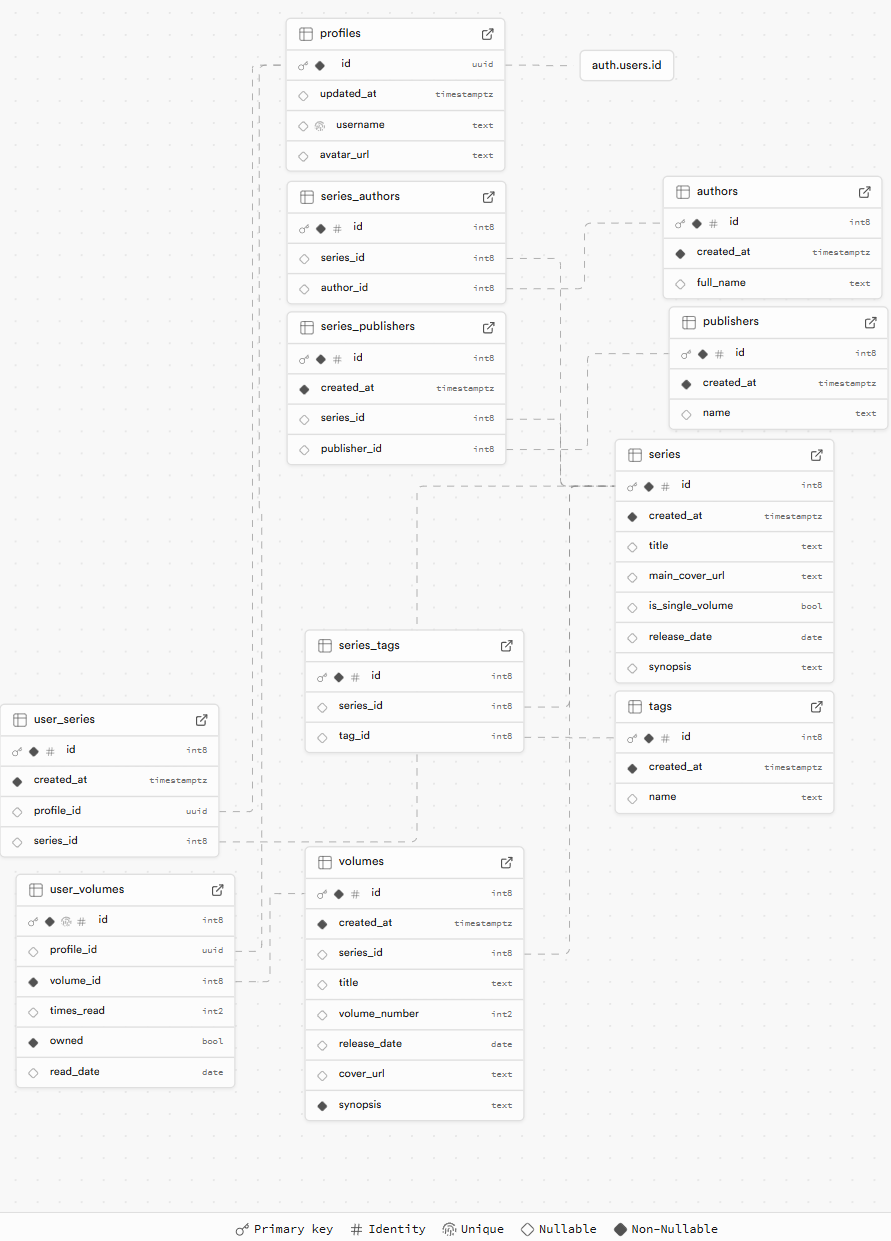
\includegraphics[width=1\textwidth]{figures/schemat1.png}
	\caption{Schemat bazy danych}
\label{Fig:schemat}
\end{figure}

\clearpage

\subsection{Normalizacja}

Normalizacja bazy danych to proces organizowania danych w taki sposób, aby zminimalizować redundancję i zapewnić 
integralność danych. Celem jest poprawienie struktury bazy w sposób, który ułatwia jej zarządzanie i utrzymanie, 
eliminując potencjalne problemy związane z nieefektywnym przechowywaniem informacji.

\subsubsection{Pierwsza postać normalna}

Pierwsza postać normalna (1NF) na podstawie kodu z listingu \ref{publicSeries}
\begin{lstlisting}[language=SQL,caption=kod tworzenia tabeli series, label={publicSeries}]
		CREATE TABLE public.series (
			id bigint GENERATED BY DEFAULT AS IDENTITY NOT NULL,
			title text NULL,
			...
			CONSTRAINT Series_pkey PRIMARY KEY (id)
		  );
\end{lstlisting}
Tabela series spełnia pierwszą postać normalną, ponieważ kolumny takie jak title zawierają atomowe 
wartości, a klucz główny (id) zapewnia unikalność każdego rekordu,

\subsubsection{Druga postać normalna}
Druga postać normalna (2NF) na podstawie kodu z listingu \ref{publicVolumes}
\begin{lstlisting}[language=SQL,caption=kod tworzenia tabeli volumes, label={publicVolumes}]
	CREATE TABLE public.volumes (
		id bigint GENERATED BY DEFAULT AS IDENTITY NOT NULL,
		series_id bigint NULL,
		title text NULL,
		...
		CONSTRAINT volumes_pkey PRIMARY KEY (id),
		CONSTRAINT volumes_series_id_fkey FOREIGN KEY (series_id) REFERENCES series(id)
		);
\end{lstlisting}
Tabela volumes spełnia drugą postać normalną, ponieważ jest w pierwszej postaci normalnej oraz 
wszystkie kolumny, które nie są częścią klucza głównego, są w pełni zależne od klucza głównego (id). 
Kolumna series\_id jest kluczem obcym, a kolumny jak title zależą od id, co eliminuje zależności 
częściowe.

\subsubsection{Trzecia postać normalna}

Trzecia postać normalna (3NF) na podstawie kodu z listingu \ref{publicUserSeries}
\begin{lstlisting}[language=SQL,caption=kod tworzenia tabeli user\_series, label={publicUserSeries}]
	CREATE TABLE public.user_series (
		id bigint GENERATED BY DEFAULT AS IDENTITY NOT NULL,
		profile_id uuid NULL,
		series_id bigint NULL,
		...
		CONSTRAINT user_series_pkey PRIMARY KEY (id),
		CONSTRAINT user_series_profile_id_fkey FOREIGN KEY (profile_id) REFERENCES profiles(id),
		CONSTRAINT user_series_series_id_fkey FOREIGN KEY (series_id) REFERENCES series(id)
	);
\end{lstlisting}
Tabela user\_series spełnia trzecią postać normalną, ponieważ jest w drugiej postaci normalnej, a 
dodatkowo nie występują zależności przejściowe. Kolumny, które nie są częścią klucza głównego, zależą 
tylko od klucza głównego (id), a nie od innych kolumn, co zapewnia brak zbędnych zależności między danymi.
Tabela ta spełnia również BCNF, ponieważ każda kolumna w niej zależy bezpośrednio od głównego identyfikatora 
(id).

\subsubsection{Czwarta postać normalna}

Czwarta postać normalna (4NF) na podstawie kodu z listingu \ref{publicSeriesAuthors}
	\begin{lstlisting}[language=SQL,caption=kod tworzenia tabeli series\_authors, label={publicSeriesAuthors}]
		CREATE TABLE public.series_authors (
		id bigint GENERATED BY DEFAULT AS IDENTITY NOT NULL,
		series_id bigint NULL,
		author_id bigint NULL,
		CONSTRAINT series_author_pkey PRIMARY KEY (id),
		CONSTRAINT series_author_author_id_fkey FOREIGN KEY (author_id) REFERENCES authors(id) ON UPDATE CASCADE ON DELETE CASCADE,
		CONSTRAINT series_author_series_id_fkey FOREIGN KEY (series_id) REFERENCES series(id) ON UPDATE CASCADE ON DELETE CASCADE
	);
\end{lstlisting}
Tabela series\_authors spełnia czwartą postać normalną, ponieważ nie zawiera zależności wielowartościowych. Relacja 
między series\_id a author\_id jest wyrażona w sposób atomowy, gdzie każda kombinacja serii i autora jest 
reprezentowana przez pojedynczy wiersz. Tabela nie wprowadza redundancji związanej z wieloma wartościami 
przypisanymi do jednej kolumny.

\subsection{Funkcje bazy danych}

Funkcje bazy danych stanowią ważny element w zarządzaniu danymi, umożliwiając efektywne wykonywanie różnych operacji 
w obrębie samej bazy danych. Funkcje PostgreSQL pozwalają na grupowanie złożonych zapytań, usprawnienie przetwarzania 
danych oraz zwiększenie wydajności operacji. Dzięki funkcjom bazy danych możliwe jest wykonywanie operacji 
specyficznych dla aplikacji bezpośrednio na poziomie bazy danych, co pozwala na zmniejszenie obciążenia aplikacji i 
serwera.

Kod przykładowej funkcji bazy danych znajduje się w listingu \ref{sqlFunction}

\begin{lstlisting}[language=SQL,caption=kod funkcji get\_volume\_by\_id, label={sqlFunction}]
	CREATE OR REPLACE FUNCTION public.get_volume_by_id(p_volume_id bigint)
	RETURNS TABLE(id bigint, title text, cover_url text, volume_number smallint, user_volume_id bigint, release_date timestamp with time zone, times_read smallint, owned boolean, synopsis text, read_date timestamp with time zone)
	LANGUAGE plpgsql
	AS $function$
	BEGIN
		RETURN QUERY
		SELECT 
			v.id,
			v.title,
			v.cover_url,
			v.volume_number,
			uv.id AS user_volume_id,
			v.release_date,
			COALESCE(uv.times_read, 0) AS times_read,
			COALESCE(uv.owned, false) AS owned,
			v.synopsis,
			uv.read_date
		FROM 
			volumes v
		LEFT JOIN 
			user_volumes uv ON v.id = uv.volume_id
		WHERE 
			v.id = p_volume_id;
	END;
	$function$;
\end{lstlisting}
Funkcja ta pozwala na podstawie identyfikatora pobrać z bazy danych informacje o wybranym tomie książki (volume), z bazy
danych. Funkcja zwraca wynik w postaci teabeli zawierającej dane o tomie oraz dodatkowe informacje związane z użytkownikiem
jeżeli są dostępne, takie jak pobrane z tabeli user\_volumes, times\_read informujące o tym ile razy użytkownik przeczytał
dany tom. Może wystąpić sytuacja, w której pobierany tom nie ma odpowiadającego rekordu w tabeli user\_volumes, ponieważ 
użytkownik nie oznaczył go jako przeczytanego ani posiadanego. W takim przypadku dane użytkownika zostaną uzupełnione 
domyślnymi wartościami, takimi jak 0 dla liczby przeczytań czy false dla statusu posiadania, co jest zrealizowane z 
wykorzystaniem funkcji COALESCE, której użycie można zaobserować w liniach 14 i 15.

\subsection{RLS (Row Level Security)}

Row-Level Security (RLS) to technika zabezpieczania danych na poziomie wierszy w bazie danych, która pozwala 
kontrolować, które wiersze są dostępne dla poszczególnych użytkowników. Dzięki RLS, można definiować zasady 
dostępu do danych w sposób precyzyjny, np. na podstawie ról użytkowników, zapewniając większą elastyczność i 
bezpieczeństwo. RLS pozwala na implementację polityk, które działają bez konieczności wprowadzania dodatkowej 
logiki w aplikacji, co upraszcza zarządzanie dostępem do danych. Przykładowa definicja polityki RLS znajduje się
w poniższym listingu \ref{rlsPolicy}

\begin{lstlisting}[language=SQL,caption=Polityka RLS "Enable delete for users based on user\_id", label={rlsPolicy}]
	alter policy "Enable delete for users based on user_id"
	on "public"."user_volumes"
	to authenticated
	using (
		(( SELECT auth.uid() AS uid) = profile_id)
	);
\end{lstlisting}
Powyższy kod przedstawia przykład polityki RLS, która umożliwia użytkownikom usuwanie danych z tabeli 
user\_volumes tylko wtedy, gdy ich identyfikator użytkownika (profile\_id) odpowiada aktualnie zalogowanemu 
użytkownikowi. Polityka ta jest przypisana do roli authenticated, co oznacza, że tylko uwierzytelnieni 
użytkownicy mogą wykonywać operację usuwania. Warunek w klauzuli using zapewnia, że dostęp do wierszy jest 
restrykcyjnie kontrolowany na poziomie wierszy, co pozwala na bezpieczne zarządzanie danymi w aplikacji bez 
konieczności implementowania dodatkowej logiki w kodzie aplikacji.


\clearpage

\section{Struktura projektu}

Aplikacja została wykonana z wykorzystaniem narzędzia Android Studio, a struktura projektu została zaprojektowana 
zgodnie z rekomendowanymi zasadami architektury MVVM (Model-View-ViewModel), co zapewnia czytelność, modułowość
oraz łatwość w utrzymaniu i rozwoju kodu. Struktura plików projektu przedstawiona jest na rysunku \ref{Fig:struktura}

\begin{figure}[ht]
	\centering
	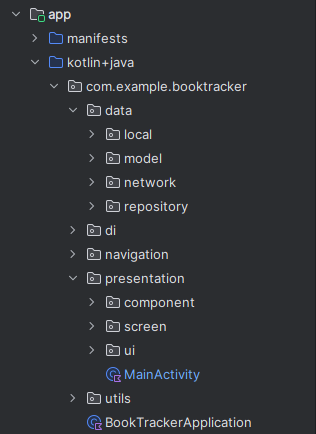
\includegraphics{figures/struktura.png}
	\caption{Struktura plików aplikacji}
\label{Fig:struktura}
\end{figure}

\subsection{Folder data}

Folder "data" pełni rolę zbiorczą dla klas i funkcji odpowiedzialnych za zarządzanie danymi, w tym ich przechowywanie 
oraz pobieranie z bazy danych.
\begin{samepage}
\begin{enumerate}[label=\alph*), leftmargin=1.25cm]
	\item Folder "local" jest przeznaczony do przechowywania danych lokalnych, takich jak tokeny autoryzacyjne, 
	ustawienia aplikacji czy inne informacje, które nie wymagają zdalnej synchronizacji, z wykorzystaniem biblioteki 
	DataStore, która zapewnia bezpieczne i efektywne przechowywanie danych w formie klucz-wartość lub preferencji,
	\item Folder "model" przechowuje klasy DTO (Data Transfer Object), które są serializowanymi obiektami 
	wykorzystywanymi do przechowywania danych pobranych z bazy danych. Klasom tym przypisuje się odpowiednie 
	struktury, które umożliwiają prawidłowe reprezentowanie i manipulowanie danymi w aplikacji,
	\item w folderze "network" przechowywane są klasy DAO (Data Access Object), które odpowiadają za komunikację z 
	bazą danych Supabase. Klasy te pełnią rolę abstrakcji, umożliwiając wykonywanie operacji na danych, takich jak 
	pobieranie, zapisywanie czy aktualizowanie rekordów, bezpośrednio w bazie. Dzięki zastosowaniu wzorca DAO, 
	operacje te są oddzielone od logiki aplikacji, co zapewnia lepszą modularność, łatwiejsze zarządzanie dostępem do 
	danych oraz umożliwia łatwiejszą wymianę technologii dostępu do danych w przyszłości,
	\item Folder "repository" jest odpowiedzialny za przechowywanie klas repozytoriów, które pełnią rolę pośredników 
	pomiędzy warstwą danych a resztą aplikacji. Repozytoria w tym folderze odpowiadają za realizację operacji dostępu 
	do różnych źródeł danych. Oddzielają one logikę biznesową aplikacji od szczegółów technicznych, zapewniając 
	łatwiejsze zarządzanie danymi oraz umożliwiając przyszłe zmiany w źródłach danych bez wpływu na resztę aplikacji. 
	Repozytoria ułatwiają testowanie, zapewniają modularność aplikacji i poprawiają jej elastyczność, umożliwiając 
	łatwą wymianę technologii dostępu do danych.
\end{enumerate}
\end{samepage}
\subsection{Folder di}

Folder "di" służy do przechowywania modułów odpowiedzialnych za konfigurację zależności aplikacji. Wykorzystuje 
bibliotekę Hilt, która umożliwia definiowanie sposobu tworzenia i dostarczania wymaganych obiektów, takich jak 
klienty API, repozytoria czy inne kluczowe komponenty. Moduły w tym folderze zapewniają centralne miejsce do 
zarządzania zależnościami, co ułatwia organizację projektu i poprawia czytelność kodu.

\subsection{Folder navigation}

Folder "navigation" zarządza całą logiką nawigacji w aplikacji, co umożliwia łatwe i efektywne przejścia pomiędzy 
ekranami. Zawiera definicję ekranów jako obiektów typu sealed class, co pozwala na centralne zarządzanie wszystkimi 
dostępnymi widokami w aplikacji.

Dzięki wykorzystaniu biblioteki navigation-compose, folder "navigation" umożliwia łatwą konfigurację tras i przejść, 
eliminując konieczność ręcznego zarządzania stanem nawigacji. Obsługuje różne scenariusze, takie jak logowanie, 
rejestracja, czy przeglądanie biblioteki, zapewniając płynność i spójność w nawigacji. 
W połączeniu z komponentem NavHost, aplikacja może efektywnie zarządzać stanem nawigacyjnym, przechodzić między 
ekranami i dostosowywać animacje przejść. Dzięki tej strukturze, aplikacja jest bardziej modularna, a logika 
nawigacyjna pozostaje łatwa do utrzymania i rozbudowy.

\subsection{Folder presentation}

Folder "presentation" zawiera pliki odpowiadające za warstwę prezentacji aplikacji. Znajdują się w nim zarówno widoki, 
które definiują interfejs użytkownika, jak i modele widoków, które dostarczają dane i logikę potrzebną do poprawnego 
działania widoków. Elementy te współpracują ze sobą, aby zapewnić spójne i przejrzyste doświadczenie użytkownika.

Folder "component" zawiera funkcje kompozycyjne, które są wykorzystywane w więcej niż jednym widoku. Przykład takiej 
funkcji przedstawiono w poniższym listingu \ref{SeriesProgressIndicator}.

\begin{lstlisting}[language=Kotlin,caption=kod funkcji SeriesProgressIndicator, label={SeriesProgressIndicator}]
	@Composable
	fun SeriesProgressIndicator(ownedProgress: Float, readingProgress: Float, height: Dp) {
		Box(
			modifier = Modifier
				.fillMaxWidth()
				.height(height)
				.background(MaterialTheme.colorScheme.surfaceVariant)
		) {
			Box(
				modifier = Modifier
					.fillMaxWidth(ownedProgress)
					.height(height)
					.background(
						MaterialTheme.colorScheme.tertiary
					)
			)
	
			Box(
				modifier = Modifier
					.fillMaxWidth(readingProgress)
					.height(height)
					.background(
						MaterialTheme.colorScheme.primary
					)
			)
		}
	}
\end{lstlisting}
Kod odpowiada za wyświetlanie paska postępu dla danej serii, który pokazuje zarówno postęp posiadanych, jak i 
aktualnie czytanych książek. Pasek jest wyświetlany w formie dwóch nałożonych na siebie prostokątów o różnych 
szerokościach, zależnych od wartości ownedProgress i readingProgress. Kod paska postępu znajduje się w folderze
"component", ponieważ jest on wykorzystywany przez komponent kart na ekranie biblioteki i w nagłówku serii, co widać
na poniższym rysunku \ref{fig:SeriesProgressIndicator}

\begin{figure}[ht]
	\centering
	\begin{subfigure}[b]{0.2\textwidth}
	  
\includegraphics[]{figures/karta.png}
	  \caption{Karta serii}
	\end{subfigure}
	\hfill
	\begin{subfigure}[b]{0.6\textwidth}
	  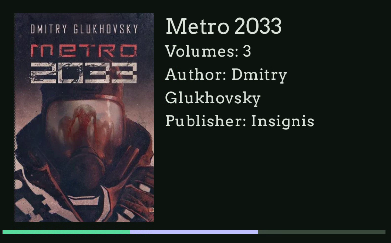
\includegraphics[]{figures/header.png}
	  \caption{Nagłówek ekranu serii}
	\end{subfigure}
	\caption{SeriesProgressIndicator wykorzystany w różnych komponentach}
	\label{fig:SeriesProgressIndicator}
\end{figure}

Kolejnym folderem jest folder "screen", który zawiera podfoldery dla poszczególnych ekranów. Każdy z tych podfolderów 
zawiera plik główny kodu ekranu, a opcjonalnie model widoku oraz folder "component" do przechowywania komponentów 
specyficznych dla danego ekranu.

Ostatni folder, "ui", dzieli się na dwa podfoldery: "theme", w którym przechowywane są pliki definiujące style 
kolorów, typografii oraz motywu aplikacji, oraz "viewmodel", zawierający pliki modeli widoków, które są współdzielone 
między kilkoma ekranami.

\subsection{Folder utils}

Folder utils zawiera funkcje pomocnicze, które wspierają różne operacje w aplikacji, takie jak walidacja danych 
wejściowych. Funkcje te są uniwersalne i mogą być wykorzystywane w różnych częściach projektu, co pozwala na unikanie 
powielania kodu. Dzięki temu zapewniają one centralizację logiki, co ułatwia utrzymanie aplikacji, poprawia jej 
czytelność oraz umożliwia łatwiejsze testowanie. Przykłady funkcji w tym folderze to metody sprawdzające poprawność 
adresu e-mail, hasła czy nazwy użytkownika. Wszystkie funkcje w utils są zaprojektowane w sposób modularny, co 
pozwala na ich elastyczne zastosowanie w całym projekcie. Przykładowa funkcja znajduje się listingu \ref{validateEmail}

\begin{lstlisting}[language=Kotlin,caption=kod funkcji validateEmail, label={validateEmail}]
	fun validateEmail(email: String, context: Context): String? {
    	val emailRegex = "^[A-Za-z0-9+_.-]+@[A-Za-z0-9.-]+\$".toRegex()
    		return if (email.isEmpty()) {
        		context.getString(R.string.email_empty)
    		} else if (!email.matches(emailRegex)) {
        		context.getString(R.string.invalid_email)
    		} else null
		}
\end{lstlisting}

\clearpage

\section{Wstrzykiwanie zależności (Dependency Injection)}

Wstrzykiwanie zależności (ang. Dependency Injection) jest jednym z kluczowych wzorców projektowych, który pomaga 
w utrzymaniu czystości kodu, jego modularności i testowalności. Wstrzykiwanie zależności odgrywa istotną rolę w 
zarządzaniu zależnościami między komponentami aplikacji, takimi jak modele widoków, repozytoria, czy usługi 
zewnętrzne.

Deklaratywne tworzenie interfejsu użytkownika w Jetpack Compose znacząco ułatwia pracę w tworzeniu aplikacji. Jednak
wraz z rosnącą złożonością, pojawia się potrzeba efektywnego zarządzania zależnościami, szczególnie w kontekście 
komponentów, które muszą współpracować ze sobą. W tym celu wykorzystuje się narzędzia do wstrzykiwania zależności, 
takie jak Hilt. Jest to nowoczesne narzędzie, które upraszcza proces zarządzania zależnościami w aplikacjach Android, 
eliminując konieczność ręcznego tworzenia i przekazywania obiektów. Hilt bazuje na popularnym rozwiązaniu o nazwie 
Dagger, które jest wykorzystywane do automatycznego i efektywnego zarządzania zależnościami w dużych aplikacjach. 
Dzięki Hilt, integracja z Androidem staje się łatwiejsza, a proces konfiguracji i wstrzykiwania zależności bardziej 
intuicyjny i mniej czasochłonny.

\subsection{Konfiguracja Hilt}

Konfiguracja Hilt dla tworzonej aplikacji polega na uruchomieniu kontenera wstrzykiwania zależności przez dodanie 
adnotacji @HiltAndroidApp do klasy aplikacji. Adnotacja ta informuje Hilt o konieczności wygenerowania kodu 
potrzebnego do zarządzania zależnościami w całej aplikacji. Przykład konfiguracji został zaprezentowany w poniższym 
listingu \ref{hiltAndroidApp}:

\begin{lstlisting}[language=Kotlin,caption=Konfiguracja Hilt w aplikacji, label={hiltAndroidApp}]
	@HiltAndroidApp
		class BookTrackerApplication: Application() {
		}
\end{lstlisting}
Dzięki zastosowaniu @HiltAndroidApp, Hilt automatycznie uruchamia kontener DI (Dependency Injection) podczas startu 
aplikacji, umożliwiając wstrzykiwanie zależności w różnych komponentach, takich jak modele widoków czy funkcje 
kompozycyjne.

Adnotacja @AndroidEntryPoint jest kluczowym elementem konfiguracji Hilt. Informuje ona system, że dana klasa 
powinna być objęta mechanizmem wstrzykiwania zależności. Dzięki temu Hilt automatycznie przygotowuje kontener DI i 
udostępnia zadeklarowane zależności, które można wstrzykiwać za pomocą adnotacji @Inject. Kod konfiguracji tej 
adnotacji w klasie głównej aplikacji został zaprezentowany w listingu \ref{hiltEntryPoint}.
\begin{lstlisting}[language=Kotlin,caption=Przykład użycia @AndroidEntryPoint w MainActivity, label={hiltEntryPoint}]
	@AndroidEntryPoint
		class MainActivity : ComponentActivity() {...}
\end{lstlisting}
Dzięki tej konfiguracji Hilt może automatycznie wstrzykiwać wszystkie zależności w komponentach podrzędnych, 
używanych w aplikacji. Ułatwia to zarządzanie złożonością kodu oraz umożliwia bardziej zwięzłą implementację 
aplikacji.

\subsection{Moduły Hilt}

Jednym z kluczowych elementów Hilt jest definiowanie modułów za pomocą adnotacji @Module. Moduły te pozwalają 
precyzyjnie określić, jakie obiekty powinny być dostarczane i w jakim cyklu życia mają istnieć. W poniższym listingu
\ref{supabaseModule} znajduje się przykład definiowania modułu dostarczającego klienta Supabase.
\begin{lstlisting}[language=Kotlin,caption=Przykład modułu klienta Supabase, label={supabaseModule}]
	@InstallIn(SingletonComponent::class)
	@Module
	object SupabaseModule {
    @Provides
    @Singleton
    fun provideSupabaseClient(): SupabaseClient {
        return createSupabaseClient(
            supabaseUrl = BuildConfig.SUPABASE_URL,
            supabaseKey = BuildConfig.API_KEY
        ) {
            install(Auth)
            install(Postgrest)
        }
    }

    @Provides
    @Singleton
    fun provideSupabaseAuth(client: SupabaseClient): Auth {
        return client.auth
    }
}
\end{lstlisting}
Adnotacja @InstallIn(...) określa, gdzie dany moduł będzie instalowany, a przez to, gdzie dostarczane zależności 
będą dostępne. Przykładowo, @InstallIn(SingletonComponent::class) z linii pierwszej wskazuje, że zależności 
zdefiniowane w module będą współdzielone w całej aplikacji. Adnotacja @Provides
Informuje Hilt, jak utworzyć daną zależność. W powyższym przykładzie funkcja provideSupabaseClient() definiuje, jak 
stworzyć instancję SupabaseClient. Adnotacja @Singleton zapewnia, że obiekt będzie tworzony tylko raz podczas działania 
aplikacji.

Innym przykładem zależności, którą można wstrzykiwać do różnych komponentów aplikacji, są lokalnie przechowywane 
dane zarządzane za pomocą DataStore. Umożliwia to scentralizowane zarządzanie preferencjami użytkownika oraz łatwy 
dostęp do nich w różnych częściach aplikacji. Moduł dla DataStore definiuje sposób dostarczania obiektu zarządzającego 
preferencjami użytkownika i jest skonfigurowany do działania w kontekście całej aplikacji. Kod tego modułu znajduje 
się w listingu \ref{DataStoreModule}.

\begin{lstlisting}[language=Kotlin,caption=Przykład modułu DataStore, label={DataStoreModule}]
@Module
@InstallIn(SingletonComponent::class)
class DataStoreModule {
    @Provides
    @Singleton
    fun provideUserPreferences(@ApplicationContext context: Context): UserPreferences {
        return UserPreferences(context)
    }
}
\end{lstlisting}

W aplikacjach opartych na wzorcu repozytorium, zarządzanie danymi odbywa się poprzez interfejs, który określa 
operacje, jakie mogą być wykonywane na danych. Implementacja tego interfejsu dostarcza konkretne mechanizmy do 
pozyskiwania danych z różnych źródeł. Wstrzykiwanie zależności w Hilt pozwala na łatwą konfigurację repozytorium, 
umożliwiając podmianę jego implementacji, co może być przydatne podczas testów lub w sytuacjach, gdzie różne źródła 
danych wymagają różnych implementacji. Przykład implementacji modułu repozytorium znajduje się w listingu 
\ref{repositoryModule}

\begin{lstlisting}[language=Kotlin,caption=Przykład modułu repozytorium SeriesRepository, label={repositoryModule}]
	@InstallIn(SingletonComponent::class)
	@Module
	abstract class SeriesRepositoryModule {
		@Binds
		@Singleton
		abstract fun bindSeriesRepository(impl: SeriesRepositoryImpl) : SeriesRepository
	}
\end{lstlisting}

\subsection{Przykłady wstrzykiwania zależności z Hilt}

Repozytorium to kluczowy komponent, który abstrahuje logikę uwierzytelniania od reszty aplikacji. W 
AuthenticationRepositoryImpl wykorzystujemy wcześniej zdefiniowane zależności, takie jak Auth i UserPreferences. 
Dzięki adnotacji @Inject Hilt automatycznie dostarcza te zależności. Kod repozytorium znajduje się w listingu 
\ref{AuthenticationRepositoryImpl}

\begin{lstlisting}[language=Kotlin,caption=Implementacja AuthenticationRepository, label={AuthenticationRepositoryImpl}]
	class AuthenticationRepositoryImpl @Inject constructor(
    private val auth: Auth,
    private val userPreferences: UserPreferences
) : AuthenticationRepository {

    override suspend fun signIn(email: String, password: String): Boolean {
        return runCatching {
            auth.signInWith(Email) {
                this.email = email
                this.password = password
            }
            true
        }.getOrDefault(false)
    }

	override suspend fun saveToken() {
        val accessToken = auth.currentAccessTokenOrNull()
        if (accessToken != null) {
            userPreferences.saveUserSession(accessToken)
        }
    }

	...

}
\end{lstlisting}
Powyższy kod przedstawia definicję klasy AuthenticationRepositoryImpl, w której wstrzykiwane są zależności: klient 
auth z modułu SupabaseModule oraz preferencje użytkownika z modułu DataStoreModule. Na przykładzie dwóch metod 
pokazano, jak można korzystać z tych zależności po ich wstrzyknięciu. Metoda signIn wykorzystuje klienta auth do 
obsługi logowania użytkownika, natomiast metoda saveToken zapisuje token sesji w preferencjach użytkownika przy 
użyciu userPreferences.

AuthViewModel wykorzystuje AuthenticationRepository, które zostało wstrzyknięte za pomocą Hilt. Dzięki temu ViewModel 
jest odpowiedzialny wyłącznie za przetwarzanie danych dla interfejsu użytkownika, bez konieczności zarządzania 
szczegółami implementacyjnymi repozytorium. Kod ViewModel przedstawiono w listingu \ref{AuthViewModelHilt}
\clearpage
\begin{lstlisting}[language=Kotlin,caption=Implementacja AuthViewModel, label={AuthViewModelHilt}]
	@HiltViewModel
	class AuthViewModel @Inject constructor(
		private val authenticationRepository: AuthenticationRepository
	): ViewModel() {
		fun onSignIn() {
        viewModelScope.launch{
            _signInResult.value = authenticationRepository.signIn(
                email = _email.value,
                password = _password.value
            )
            if (_signInResult.value!!) {
                authenticationRepository.saveToken()
            }
        }
    }
	... 
	}
\end{lstlisting}
Dzięki Hilt, AuthViewModel otrzymuje AuthenticationRepository bez konieczności jego ręcznego tworzenia. To pozwala 
na oddzielenie logiki aplikacji od szczegółów implementacyjnych repozytorium. W przypadku potrzeby zmiany na inne
źródło danych wystarczy zmienić tylko moduł Hilt. AuthViewModel pozostałby bez zmian, ponieważ nie jest odpowiedzialny 
za tworzenie instancji repozytorium.

Funkcja SignInScreen odpowiada za wyświetlenie ekranu logowania. Dzięki funkcji hiltViewModel() instancja 
AuthViewModel jest automatycznie tworzona i dostarczana przez Hilt. W ten sposób uniknięto ręcznego zarządzania 
cyklem życia ViewModel, a kod staje się bardziej przejrzysty. Kod funkcji znajduje się w listingu \ref{SignInScreenHilt}
\begin{lstlisting}[language=Kotlin,caption=Implementacja AuthViewModel, label={SignInScreenHilt}]
	@Composable
	fun SignInScreen(
		toSignUpScreen: (() -> Unit),
		toHomeScreen: (() -> Unit),
		signInViewModel: AuthViewModel = hiltViewModel(),
	) {
		...
	}
\end{lstlisting}
W tej funkcji signInViewModel jest wykorzystywany do zarządzania stanem ekranu i obsługi zdarzeń, takich jak próba 
logowania. Dzięki temu kod w funkcji Composable pozostaje skupiony na interfejsie użytkownika.

\clearpage

\section{MVVM (Model-View-ViewModel)}

Model-View-ViewModel to popularny wzorzec architektoniczny stosowany w tworzeniu aplikacji, który pomaga w 
organizacji kodu i rozdzieleniu odpowiedzialności pomiędzy różne warstwy aplikacji. Jego głównym celem
jest zwiększenie modularności, łatwości testowania oraz oddzielenie logiki biznesowej od interfejsu użytkownika.
\begin{samepage}
\begin{enumerate}[label=\alph*), leftmargin=1.25cm]
	\item Model reprezentuje warstwę danych i logiki biznesowej. Jest odpowiedzialny za zarządzanie danymi,
	które mogą pochodzić z różnych źródeł, takich jak bazy danych, API czy pliki lokalne. Model nie zawiera
	żadnej logiki związanej z interfejsem użytkownika ani sposobem prezentacji danych,
	\item View (Widok) odpowiada za warstwę prezentacji. Widok to interfejs użytkownika (UI), który jest
	odpowiedzialny za wyświetlenie danych i odbieranie interakcji od użytkownika. Widok powinien jedynie
	reagować na dane dostarczane przez ViewModel. W android widokiem są komponenty Jetpack Compose,
	\item ViewModel to warstwa pomiędzy modelem a widokiem. pobiera dane z modelu i przekształca je
	w taki sposób, aby były gotowe do wyświetlenia w widoku. Ponadto zarządza stanem widoku (np. przechowywaniem
	stanu aplikacji w przypadku zmiany orientacji ekranu).
\end{enumerate}
\end{samepage}

\subsection{Model}
W podrozdziale "Model" omówione zostaną kluczowe komponenty warstwy modelu w architekturze MVVM, odpowiedzialnej za 
zarządzanie danymi. Zostaną przedstawione takie elementy jak DTO (Data Transfer Object), DAO (Data Access Object) 
oraz repozytoria, które umożliwiają efektywne przechowywanie, dostęp i przetwarzanie danych, a także komunikację z 
zewnętrznymi źródłami, takimi jak bazy danych czy API.

\subsubsection{Data Transfer Object}
Data Transfer Object (DTO) to wzorzec projektowy, który służy do przenoszenia danych między różnymi warstwami 
aplikacji. DTO są zazwyczaj prostymi obiektami, które zawierają dane, ale nie posiadają logiki biznesowej. Głównym 
celem DTO jest przenoszenie danych w sposób efektywny i umożliwiający łatwe zarządzanie. Przykładowy kod DTO jest 
zaprezentowany w poniższym listingu \ref{SeriesDTO}

\begin{lstlisting}[language=Kotlin,caption=Data Transfer Object Series, label={SeriesDTO}]
@Serializable
data class Series(
    val id: Int,
    val created_at: String,
    val title: String,
    val main_cover_url: String,
    val is_single_volume: Boolean,
    val release_date: LocalDate,
    val synopsis: String,
    var total_volumes_released: Int,
    var is_following: Boolean
)
\end{lstlisting}
Powyższy kod przedstawia klasę Series. Zawiera ona podstawowe informacje o serii książek, takie jak unikalny 
identyfikator (id), tytuł serii (title), data wydania (release\_date), streszczenie fabuły (synopsis), a także 
dodatkowe informacje jak liczba wydanych tomów (total\_volumes\_released) oraz status obserwowania serii przez 
użytkownika (is\_following). Wszystkie te dane są przechowywane w formacie, który może być łatwo przesyłany między 
różnymi warstwami aplikacji, takimi jak repozytoria, ViewModel czy interfejs użytkownika.

Klasa Series jest oznaczona adnotacją @Serializable, co sprawia, że może być łatwo przekształcana do i z formatu 
JSON. Serializacja jest kluczowa, ponieważ w przypadku aplikacji komunikujących się z zewnętrznymi API, jak np. 
Supabase, dane są często przesyłane w formacie JSON. Aby odpowiedź z API mogła zostać zamapowana na obiekt w 
Kotlinie, musi być ona odpowiednio zserializowana.

\subsubsection{Data Access Object}
Warstwa dostępu do danych (DAO - Data Access Object) odpowiada za komunikację z bazą danych lub zewnętrznymi 
źródłami danych, takimi jak API. Zastosowanie wzorca DAO pozwala na izolowanie logiki dostępu do danych od reszty 
aplikacji, co ułatwia zarządzanie kodem, testowanie oraz utrzymanie aplikacji. Klasa DAO odpowiada za wykonanie 
operacji związanych z pobieraniem, zapisywaniem lub aktualizowaniem danych w bazie danych lub serwisie zewnętrznym.
Przykładowy kod DAO znajduje się w poniższym listingu \ref{SeriesDao}

\begin{lstlisting}[language=Kotlin,caption=Data Transfer Object Series, label={SeriesDao}]
	class SeriesDao @Inject constructor(private val supabaseClient: SupabaseClient) {

    suspend fun getSeriesPaginated(offset: Int, limit: Int, searchQuery: String): List<Series> =
        withContext(Dispatchers.IO) {
            supabaseClient.postgrest.rpc(
                "get_series_paginated", seriesParams(offset, limit, searchQuery)
            ).decodeList<Series>()
        }
		// Inne metody
		suspend fun getAllUserVolumes(seriesId: Int): List<Volume> = withContext(Dispatchers.IO) {
        val response = supabaseClient.postgrest.rpc(
            "get_user_volumes_by_series",
            mapOf("p_series_id" to seriesId)
        ).decodeList<Volume>()
        response
    }
		suspend fun insertUserVolume(volumeToInsert: VolumeToInsert): Int? =
        withContext(Dispatchers.IO) {
            runCatching {
                val result = supabaseClient.from("user_volumes")
                    .upsert(volumeToInsert, onConflict = "profile_id, volume_id") {
                        select(columns = Columns.list("id"))
                    }.decodeList<VolumeResponse>()
                result.firstOrNull()?.id
            }.onFailure { e ->
                e.message?.let { Log.e("InsertError", it) }
            }.getOrNull()
        }
    suspend fun updateUserVolume(volumeToUpdate: VolumeToUpdate): Boolean =
        withContext(Dispatchers.IO) {
            runCatching {
                supabaseClient.from("user_volumes").update(volumeToUpdate) {
                    filter { eq("id", volumeToUpdate.id) }
                }
                true
            }.onFailure { e ->
                e.message?.let { Log.e("InsertError", it) }
            }.getOrDefault(false)
        }
    suspend fun deleteUserVolume(userVolumeId: Int): Boolean =
        withContext(Dispatchers.IO) {
            runCatching {
                supabaseClient.from("user_volumes").delete() {
                    filter { eq("id", userVolumeId) }
                }
                true
            }.onFailure { e ->
                e.message?.let { Log.e("InsertError", it) }
            }.getOrDefault(false)
        }
	}
\end{lstlisting}
W powyższym listingu przedstawiono implementację klasy SeriesDao oraz części jej metod. Metoda getSeriesPaginated 
odpowiada za pobieranie z bazy danych listy serii książek z zastosowaniem paginacji, co pozwala uniknąć przeciążenia 
aplikacji poprzez jednoczesne pobieranie zbyt dużych zbiorów danych. Odpowiedź z bazy danych jest następnie 
dekodowana do instancji klasy Series, która jest serializowanym obiektem reprezentującym serię książek. Reszta metod 
przedstawionych w powyższym listingu ma na celu realizację operacji CRUD (Create, Read, Update, Delete) na danych 
użytkownika w kontekście tomów, które posiada w swojej kolekcji, lub które przeczytał.

\subsubsection{Repozytorium}

Repozytoria w architekturze MVVM odpowiadają za dostęp do danych, oddzielając logikę aplikacji od szczegółów 
implementacji. Przykład repozytorium znajduje się na poniższym listingu \ref{seriesRepository}

\begin{lstlisting}[language=Kotlin,caption=Interfejs SeriesRepository, label={seriesRepository}]
	interface SeriesRepository {
		suspend fun getSeries(page: Int, pageSize: Int, searchQuery: String): List<Series>
		suspend fun getFollowedSeries(page: Int, pageSize: Int, sortByDate: Boolean, showFinished: Boolean): List<FollowedSeries>
		suspend fun getSeriesInfo(seriesId: Int): SeriesInfo
		suspend fun getSeriesById(seriesId: Int): Series
		suspend fun getVolumes(seriesId: Int): List<Volume>
		suspend fun getVolume(volumeId: Int): Volume
		suspend fun followSeries(seriesId: Int): Boolean
		suspend fun unfollowSeries(seriesId: Int): Boolean
		suspend fun insertUserVolume(volumeToInsert: VolumeToInsert): Int?
		suspend fun updateUserVolume(volumeToUpdate: VolumeToUpdate): Boolean
		suspend fun deleteUserVolume(userVolumeId: Int): Boolean
		suspend fun getUpcomingVolumes(page: Int, pageSize: Int): List<UpcomingVolume>
	}
\end{lstlisting}
Interfejs SeriesRepository, definiuje kontrakt dla operacji związanych z zarządzaniem seriami książek oraz ich 
tomami. Interfejs ten zawiera metody do pobierania list danych (getSeries, getFollowedSeries), wykonywania operacji 
CRUD (followSeries, unfollowSeries, insertUserVolume, updateUserVolume, deleteUserVolume) oraz uzyskiwania 
szczegółowych informacji (getSeriesInfo, getSeriesById, getVolume)

Implementacją tego interfejsu jest klasa SeriesRepositoryImpl, która korzysta z DAO (SeriesDao) do bezpośredniej 
komunikacji z bazą danych. Kod tej klasy znajduje się poniższym listingu \ref{seriesRepositoryImpl}
\begin{lstlisting}[language=Kotlin,caption=Interfejs SeriesRepository, label={seriesRepositoryImpl}]
class SeriesRepositoryImpl @Inject constructor(private val seriesDao: SeriesDao) :
    SeriesRepository {

    override suspend fun getSeries(page: Int, pageSize: Int, searchQuery: String): List<Series> {
        val offset = page * pageSize
        return seriesDao.getSeriesPaginated(offset, pageSize, searchQuery)
    }

	//inne metody

	override suspend fun getVolumes(seriesId: Int): List<Volume> {
        return seriesDao.getAllUserVolumes(seriesId)
    }

	override suspend fun insertUserVolume(volumeToInsert: VolumeToInsert): Int? {
        return seriesDao.insertUserVolume(volumeToInsert)
    }

    override suspend fun updateUserVolume(volumeToUpdate: VolumeToUpdate): Boolean {
        return seriesDao.updateUserVolume(volumeToUpdate)
    }

    override suspend fun deleteUserVolume(userVolumeId: Int): Boolean {
        return seriesDao.deleteUserVolume(userVolumeId)
    }
}
\end{lstlisting}
W implementacji klasy SeriesRepositoryImpl można zauważyć bezpośrednie wykorzystanie metod zdefiniowanych w klasie 
SeriesDao, które zostały szczegółowo omówione w poprzednim podrozdziale \textit{Data Access Object}. Przykładowo, 
metoda getSeries oblicza odpowiedni offset dla paginacji i deleguje zadanie pobrania danych do metody 
getSeriesPaginated z klasy DAO. Dzięki temu logika biznesowa i techniczne szczegóły operacji na danych są 
odseparowane.

Dzięki zastosowaniu wzorca repozytorium, logika dostępu do danych, zaimplementowana w warstwie DAO, zostaje 
odseparowana od reszty aplikacji, co ułatwia testowanie i możliwość modyfikacji w przyszłości. Klasa 
SeriesRepositoryImpl pełni tutaj rolę pośrednika, który wykorzystuje DAO do wykonywania operacji na danych, 
jednocześnie zapewniając, że pozostałe warstwy aplikacji są odizolowane od szczegółów implementacyjnych, takich jak 
konkretne zapytania do bazy danych.

\subsection{ViewModel}

ViewModel w Jetpack Compose pełni kluczową rolę w zarządzaniu stanem aplikacji i logiką biznesową w sposób 
bezpieczny dla cyklu życia komponentów. W ViewModelu przechowywane są dane aplikacji, które mogą być dynamicznie 
modyfikowane i aktualizowane w odpowiedzi na różne zdarzenia, takie jak akcje użytkownika czy zmiany w danych 
zewnętrznych. Stan jest zazwyczaj reprezentowany za pomocą obiektów takich jak StateFlow lub LiveData, które 
umożliwiają efektywne i reaktywne przekazywanie informacji do interfejsu użytkownika. Przykładowy kod
ViewModelu znajduje się w poniższym listingu \ref{LibraryViewModel}

\begin{lstlisting}[language=Kotlin,caption=Przykład klasy ViewModel dla biblioteki użytkownika, label={LibraryViewModel}]
	@HiltViewModel
	class LibraryViewModel @Inject constructor(
		private val seriesRepository: SeriesRepository,
		private val userPreferences: UserPreferences
	) :
		ViewModel() {
	
		private val _userSeries = MutableStateFlow<List<FollowedSeries>>(emptyList())
		val userSeries: StateFlow<List<FollowedSeries>> = _userSeries

		...

		private val _libraryTabsState = MutableStateFlow(0)
		val libraryTabsState: StateFlow<Int> = _libraryTabsState
		
		private var currentPage = 0
		private val pageSize = 20
		private var isLoading = false
		private var isLastPage = false

		private val _sortByDate = MutableStateFlow(true)
		val sortByDate: StateFlow<Boolean> = _sortByDate
	
		private val _showFinished = MutableStateFlow(false)
		val showFinished: StateFlow<Boolean> = _showFinished
	
		fun switchTab(index: Int) {
			_libraryTabsState.value = index
		}

		fun fetchFollowedSeries() {
			if (isLoading || isLastPage) return
	
			viewModelScope.launch {
				isLoading = true
				runCatching {
					seriesRepository.getFollowedSeries(
						page = currentPage,
						pageSize = pageSize,
						sortByDate = _sortByDate.value,
						showFinished = _showFinished.value
					)
				}.onSuccess { newSeries ->
					if (newSeries.size < pageSize) {
						isLastPage = true
					}
					_userSeries.value += newSeries
					currentPage++
				}.onFailure { e ->
					Log.e("SeriesViewModel", "Error fetching series", e)
				}.also {
					isLoading = false
				}
			}
		}

		...

		fun updateSorting(sortByDate: Boolean) {
			_sortByDate.value = sortByDate
			viewModelScope.launch {
				userPreferences.saveSortBy(sortByDate)
				refreshSeries()
			}
		}
	
		fun updateShowFinished(showFinished: Boolean) {
			_showFinished.value = showFinished
			viewModelScope.launch {
				userPreferences.saveShowFinished(showFinished)
				refreshSeries()
			}
		}
	}
\end{lstlisting}
Powyższy listing przedstawia klasę LibraryViewModel, do której wstrzykiwane są instancje SeriesRepository oraz 
UserPreferences. Klasa ta pełni rolę pośrednika między warstwą danych a interfejsem użytkownika, zarządzając 
stanem oraz logiką biznesową związaną z biblioteką użytkownika. W tej implementacji wykorzystano mechanizm 
StateFlow z biblioteki Kotlin Coroutines, który pozwala na zarządzanie stanem aplikacji w sposób asynchroniczny 
i reaktywny.

Mechanizm StateFlow, oparty na Flow, umożliwia efektywne zarządzanie przepływem danych w aplikacji. Dzięki 
asynchroniczności, wszystkie operacje wykonywane w tle nie blokują głównego wątku aplikacji, co przyczynia się 
do płynności działania aplikacji. Dodatkowo, zmiany w strumieniach są automatycznie propagowane do obserwatorów, 
co upraszcza logikę interfejsu użytkownika i eliminuje potrzebę ręcznego zarządzania stanem.

W klasie LibraryViewModel zdefiniowano kilka zmiennych, które reprezentują strumienie stanu, takich jak 
\_userSeries, \_libraryTabsState, \_sortByDate oraz \_showFinished. Prefiks \_ w nazwach zmiennych oznacza, że 
są to zmienne wewnętrzne, modyfikowane wyłącznie w obrębie samej klasy. Na przykład, \_userSeries przechowuje 
listę obserwowanych serii, która jest dynamicznie aktualizowana na podstawie danych zwracanych przez 
repozytorium. Z kolei zmienne, które nie mają prefiksu \_, są publicznymi getterami, które 
udostępniają stan zdefiniowany w zmiennych wewnętrznych, ale tylko do odczytu. Dzięki temu inne klasy mogą 
jedynie obserwować zmiany stanu, bez możliwości jego bezpośredniej modyfikacji. Takie podejście gwarantuje 
enkapsulację oraz pełną kontrolę nad procesem zarządzania danymi.

Funkcje w ViewModelu są zazwyczaj zaprojektowane jako bezstanowe operacje lub metody, które modyfikują 
wewnętrzne strumienie stanu. Na przykład w klasie LibraryViewModel funkcje takie jak fetchFollowedSeries 
odpowiadają za pobieranie danych z repozytorium i aktualizowanie odpowiednich zmiennych stanu, takich jak 
\_userSeries. Dzięki zastosowaniu viewModelScope operacje te są wykonywane asynchronicznie, co zapobiega 
blokowaniu głównego wątku aplikacji.

\subsection{View}

Widoki odpowiadają za prezentację danych użytkownikowi i reagowanie na jego interakcje. W Jetpack Compose widoki 
są definiowane za pomocą funkcji kompozycyjnych, które w sposób deklaratywny opisują strukturę interfejsu 
użytkownika. Dzięki połączeniu z warstwą ViewModel, widoki mogą dynamicznie aktualizować swoją zawartość w 
odpowiedzi na zmiany stanu aplikacji, zachowując jednocześnie prostotę i czytelność implementacji. W poniższym
listingu \ref{LibraryScreen} przedstawiona jest przykładowa implementacja widoku.
\begin{lstlisting}[language=Kotlin,caption=Kod widoku LibraryScreen , label={LibraryScreen}]
	@Composable
	fun LibraryScreen(
		seriesViewModel: SeriesViewModel,
		libraryViewModel: LibraryViewModel = hiltViewModel(),
		toSeriesScreen: (() -> Unit),
		toVolumeScreen: (() -> Unit)
	) {
		val libraryTabsState by libraryViewModel.libraryTabsState.collectAsState()
		val sortByDate by libraryViewModel.sortByDate.collectAsState()
		val showFinished by libraryViewModel.showFinished.collectAsState()
		var showBottomSheet by remember { mutableStateOf(false) }
		val sheetState = rememberModalBottomSheetState()
	
		Box(modifier = Modifier.fillMaxSize()) {
			Column(
				horizontalAlignment = Alignment.CenterHorizontally,
				verticalArrangement = Arrangement.Top
			) {
				TabRow(
					state = libraryTabsState,
					titles = listOf(
						stringResource(R.string.library).uppercase(),
						stringResource(R.string.upcoming)
					),
					onTabClick = { newIndex ->
						libraryViewModel.switchTab(newIndex)
					})
				if (libraryTabsState == 0) {Library(seriesViewModel, libraryViewModel, toSeriesScreen)} 
				else if (libraryTabsState == 1) {Upcoming(seriesViewModel, libraryViewModel, toSeriesScreen, toVolumeScreen)}
			}
			if (libraryTabsState == 0) {
				FloatingActionButton(
					modifier = Modifier
						.align(Alignment.BottomEnd)
						.padding(16.dp),
					onClick = { showBottomSheet = true }) {
					Icon(painterResource(R.drawable.filter_list), contentDescription = null)
				}
			}
			if (showBottomSheet) {
				FilterBottomSheet(
					sheetState,
					{ showBottomSheet = false },
					sortByDate,
					showFinished,
					onSortByChange = {
						libraryViewModel.updateSorting(!sortByDate)
						libraryViewModel.refreshSeries()
					},
					onShowFinishedChange = {
						libraryViewModel.updateShowFinished(!showFinished)
						libraryViewModel.refreshSeries()
					})
			}
		}
	}
\end{lstlisting}
Powyższy kod przedstawia widok LibraryScreen, który integruje dane dostarczane przez ViewModele z interfejsem 
użytkownika w Jetpack Compose. Funkcja kompozycyjna korzysta z LibraryViewModel oraz SeriesViewModel, aby 
zapewnić dostęp do stanów i logiki związanej z biblioteką użytkownika. Wykorzystanie metody collectAsState() 
pozwala na automatyczne odświeżanie elementów interfejsu w odpowiedzi na zmiany w strumieniach stanu.

Zmienna libraryTabsState oraz pozostałe stany, takie jak sortByDate i showFinished, są przekazywane do widoku 
bezpośrednio jako obserwowalne strumienie danych. Dzięki temu widok jest w pełni zsynchronizowany z aktualnym 
stanem aplikacji, a wszelkie zmiany wprowadzane w ViewModelu natychmiast znajdują odzwierciedlenie w interfejsie 
użytkownika. Podejście to pozwala na uproszczenie logiki w samym widoku oraz minimalizuje ryzyko problemów 
związanych z ręcznym zarządzaniem stanem.

Widok został zaprojektowany modularnie, z wykorzystaniem elementów takich jak TabRow, które odpowiadają za 
przełączanie między zakładkami. Przykład pokazuje również zastosowanie przycisku FloatingActionButton, który 
umożliwia użytkownikowi otwarcie dolnego arkusza (BottomSheet) służącego do filtrowania wyników. Warto zauważyć, 
że funkcje takie jak switchTab() oraz updateSorting() i updateShowFinished() są wywoływane bezpośrednio z widoku, 
co upraszcza przekazywanie akcji użytkownika do warstwy logiki biznesowej.

\clearpage

\section{Nawigacja}

\clearpage

\section{Podsumowanie}

Autor za wkład własny uważa stworzenie struktury bazy danych, funkcji PostgreSQL do pobierania z niej danych i 
zaprogramowanie aplikacji na system android 

\clearpage

\addcontentsline{toc}{section}{Literatura}

\begin{thebibliography}{4}
	\bibitem{} https://kotlinlang.org/docs/home.html
	\bibitem{} https://supabase.com/docs/reference/kotlin/introduction
	\bibitem{} https://developer.android.com/develop/ui/compose/documentation
	\bibitem{} https://m3.material.io/
\end{thebibliography}

\clearpage

\makesummary

\end{document} 
